\chapter{Déploiement}

\section{Methodology}
For the machine learning model creation we followed the Knowledge Discovery in Databases (\textit{KDD})\cite{3} methodology which is an iterative multi-stage process for extracting useful information from databases. This process is a road map with multiple stages that emphasises on early decisions and choices we make showing how important planning can lead to a successful and well managed project. This methodology was invented by Oussama Fayyad back in the 1996.

\begin{figure}[h!]
    \centering
    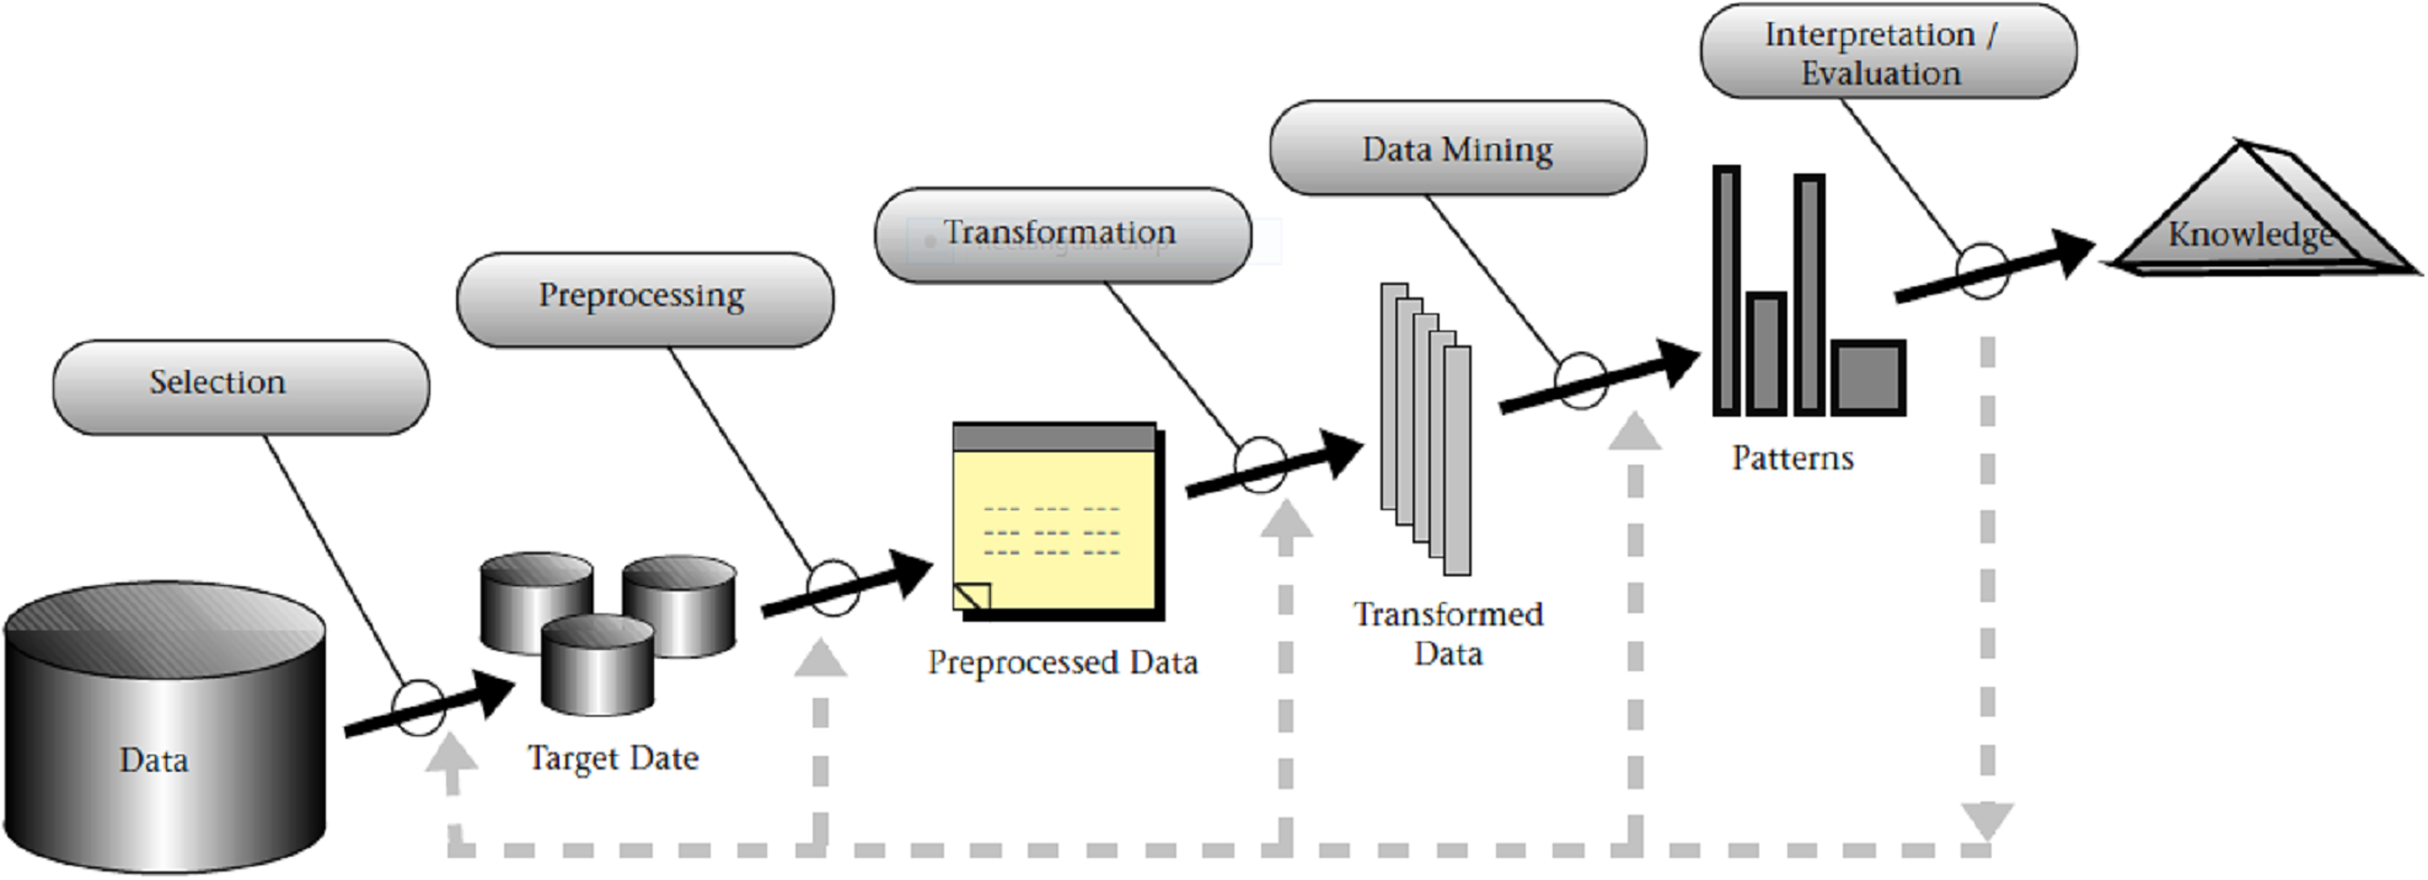
\includegraphics{chapters/KDD.png}
    \caption{Knowledge Discovery in Databases Methodology}
    \label{fig:Knowledge Discovery in Databases Methodology}
\end{figure}

\clearpage

\subsection{Selection}

The initial graphs were gathered from the \href{https://networkrepository.com}{network repository} . In addition to the different characteristics of each graph.
\\
\\
We then used these graphs to run our work product on different environments, gather the results of each test and save them into different files using the \textit{Writer} module.
\\
\\
We also gathered the characteristics from each machine to be used in our model.
\\
\\
\begin{figure}[h!]
    \centering
    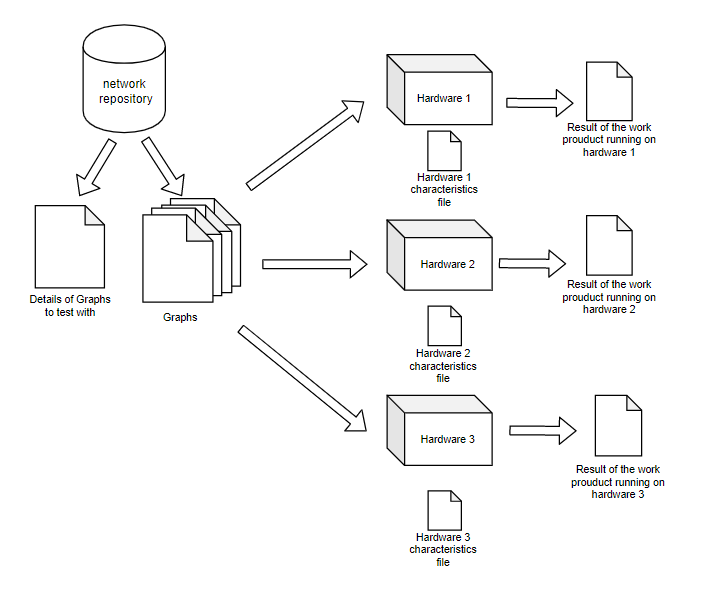
\includegraphics{chapters/Selection.png}
    \caption{Selection stage}
    \label{fig:Selection stage}
\end{figure}
\FloatBarrier
\subsection{Preprocessing and feature selection}

\subsubsection{Data integration}

After the selection phase, we joined our results into one data store from which we are going to extract knowledge.
\\
\\
We joined files containing details on graphs and files containing results of our work product by graph name.
\\
\\
We joined files containing information of the hardware characteristics and our result files by hardware name.
\begin{figure}[h!]
    \centering
    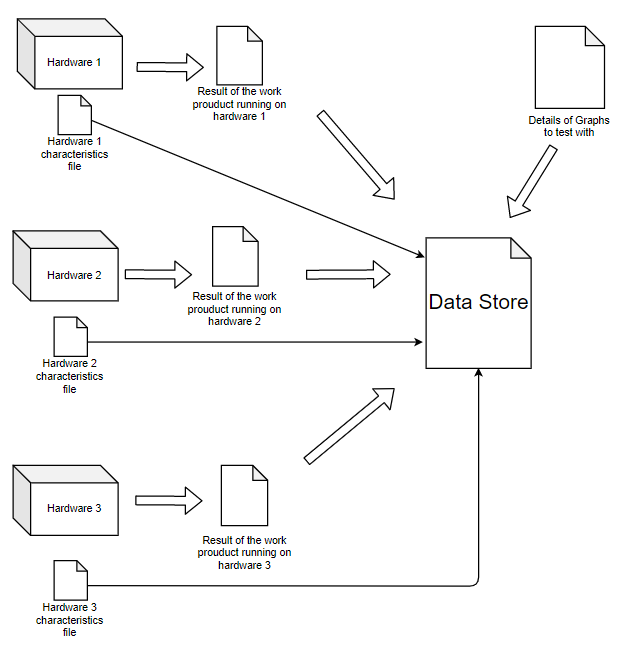
\includegraphics{chapters/merge data.png}
    \caption{Data integration}
    \label{fig:Data integration}
\end{figure}
\FloatBarrier

\subsubsection{Naming conventions}

We started by naming our different features using a certain convention ( all our features are written in \textit{Pascal Case} with spaces between words. Each column not following this convention will be renamed.

\subsubsection{Dividing features based on complexity}

After naming our features we started classifying them based on their complexity. We divided our features into three groups

\begin{itemize}
    \item Available features : these are features that can be easily determined and are generally gathered from our initial data set, such as :
    \begin{itemize}
        \item \textit{Number Of Threads}: This feature is used implicitly by the Graph Strategy prediction model 
        \item \textit{Number Of Edges $\lvert\mathcal{E}\rvert$}: This can be calculated by only counting the lines on the file, and can even be estimated in $\mathcal{O}(1)$ by viewing the graph file size and reading some random lines.
        \item \textit{Number Of Nodes $\lvert\mathcal{V}\rvert$}: We set $n\leftarrow 0$, we then read each vertex $u$ on the file, and set $n\leftarrow \max(n,u+1).$ The number of nodes is then $n$
        \item \textit{Density}:It is equal to $\frac{\lvert\mathcal{E}\rvert}{\lvert\mathcal{V}\rvert(\lvert\mathcal{V}\rvert-1)}$

    \end{itemize}
    \item Calculable features : these features can be calculated from the graph file without creating the graph, such as : 
        \begin{itemize}
            \item Contains all Available features.
            \item \textit{Max Degree}: This can be calculated by creating a vector of size $\lvert\mathcal{V}\vert$ and for each line $u \quad v$ of the graph file we set $T[u]\leftarrow T[u]+1.$ the max degree is then $\max_{u} T[u]$
            \item \textit{Min Degree}: Same as the max degree, but we return $\min_{u} T[u]$
            \item \textit{Average Degree}: Same as the max degree, but we return $\frac{\sum_u T[u]}{\lvert\mathcal{V}\rvert}$
    \end{itemize}
    \item Hard features : These are features requires the creation of the graph, or are simply computationally not feasible, such as :
    \begin{itemize}
        \item \textit{Assortativity}
        \item \textit{Number Triangles}: The fastest possible algorithm\cite{8} has complexity $\mathcal{O}(\lvert \mathcal{V}\rvert ^\omega)$\footnote{$\omega\approx 2.376$ is the fast matrix multiplication exponent.}.So it is not feasible to calculate the number of triangles given the size of considered graphs, we can only do some estimations of this features.
        \item \textit{Average Number Of Triangles}, \textit{Max Number Of Triangles}, \textit{Average Clustering Coefficient}, \textit{Fraction Closed Triangles}: Are all directly related to the number of triangles, so they share its computational complexity.
        \item \textit{Max K Core}: can be calculated in linear time $\mathcal{O}(\lvert\mathcal{V}\rvert+\lvert\mathcal{E}\rvert),$ but only if the graph is created, which is not possible in our case, because we are going to estimate the best strategy without creating the graph itself!. 
    
    \end{itemize}
\end{itemize}

\subsubsection{Imputing memory missing values}

By knowing at least the result when we run our test on a specific hardware with a graph using a fixed number of threads, we can predict the ram usage of other test results on the same hardware and same graph using linear regression with a good precision. This has been observed initially in the previous chapter.
\\
\\
For that reason, we will complete missing memory values using linear regression for each graph and hardware couple, these diagrams represent that process : 

\begin{figure}[h!]
    \centering
    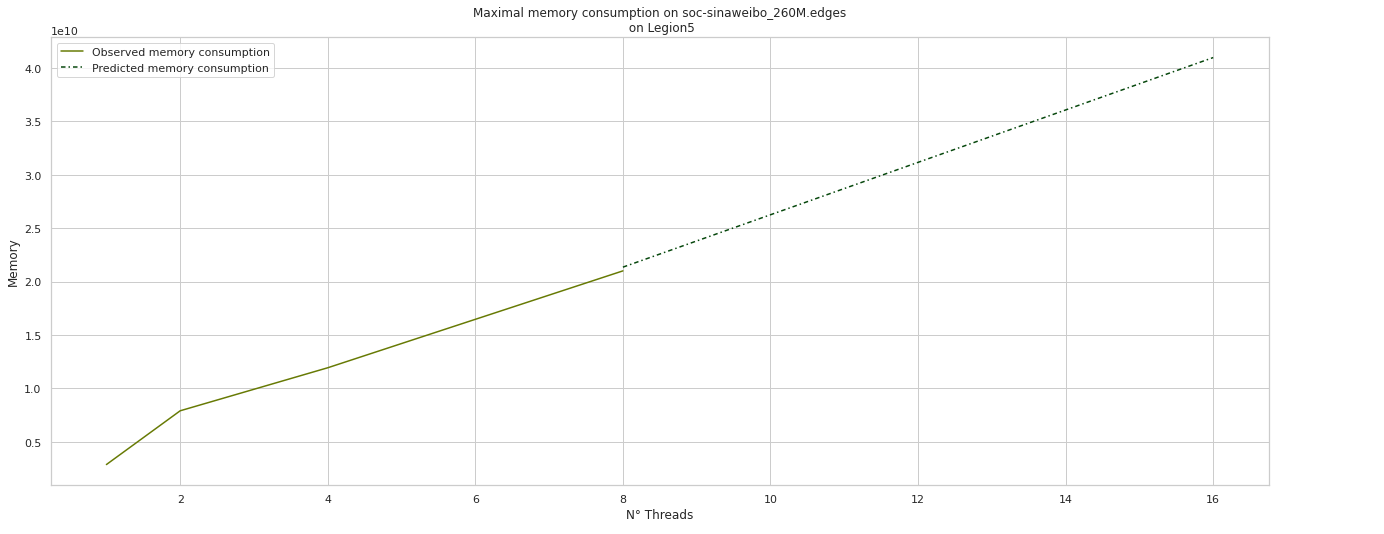
\includegraphics[width=1.0\textwidth]{images/260_legion5.png}
    \caption{Linear regression on ideapad machine}
    \label{fig:Linear regression on ideapad machine}
\end{figure}


\begin{figure}[h!]
    \centering
    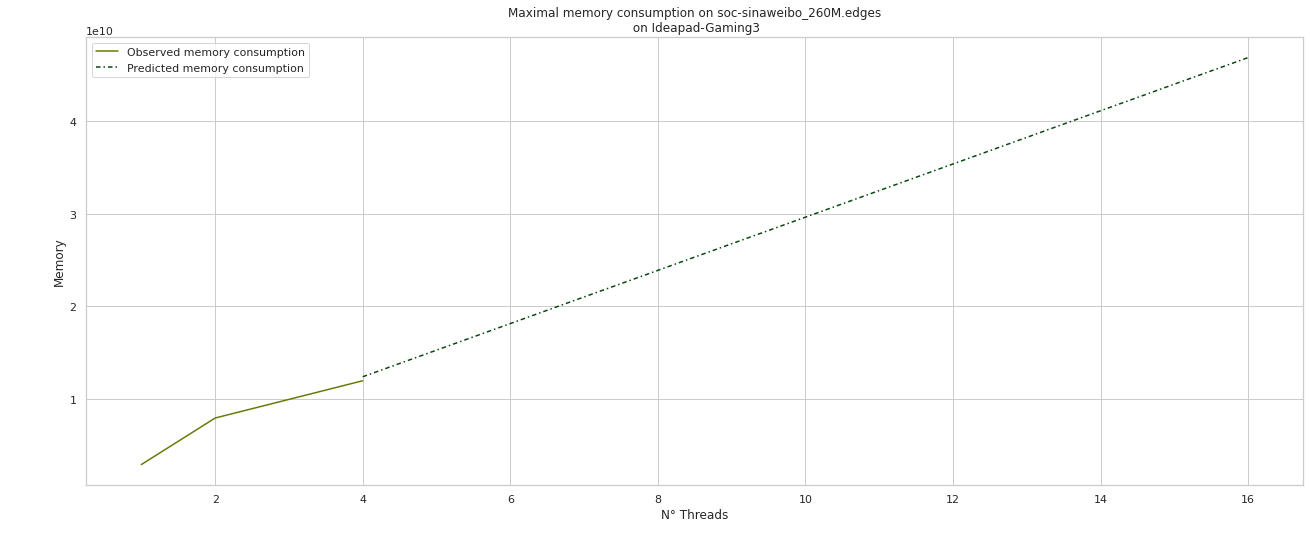
\includegraphics[width=1.0\textwidth]{images/260_ideapad.png}
    \caption{Linear regression on legion5 machine}
    \label{fig:Linear regression on legion5 machine}
\end{figure}

\subsection{Transformation}

In this step we transformed a few of our values to ensure easier manipulation and readability later on.  
    \begin{itemize}
        \item we converted all time fields into \textit{seconds}
        \item we converted the memory to \textit{Gigabyte}
    \end{itemize}

\subsection{Data Mining}

\subsubsection{Data Mining Memory and time}

We started by building two models. One to predict the approximate time the graph creation and the other to predict the memory used. These models will later be used in our final model to predict the best number of threads we can use.

\subsubsection{Predicting number of threads that maximizes memory usage}

Having the Time Model and the memory model, we can now search for the optimal number of threads that minimizes the graph creation time without exhausting the memory. So we created a Graph Strategy Prediction model that predicts the number of threads using the following algorithm:
\\
\\

\begin{algorithm}
\caption{Number of threads prediction}\label{alg:cap}
    \begin{algorithmic}
        \State $nbThreadsBest \gets 1$
        \State $timeUsedMin \gets +\infty$
        \While{$nbThreads \leq limit$}
            \State $memoryUsed \gets memoryModel(nbThreads)$
            \State $timeUsed \gets timeModel(nbThreads)$
            \If{$timeUsed < timeUsedMin$}
                \If {$MemoryUsed < memoryLimit$}
                    \State $timeUsedMin \gets timeUsed$
                    \State $nbThreadsBest \gets nbThreads$
                \EndIf
            \EndIf
        \EndWhile
    \end{algorithmic}
\end{algorithm}


\subsection{Model Selection}
Initially We selected the following $4$ models: 
\begin{itemize}
\item Linear Support vector Machine:  It gives us the flexibility to define how much error is acceptable in our model and will find an appropriate line (or hyperplane in higher dimensions) to fit the data.
\item Linear Regression: The model tries to fit the data into one linear function and make certain predictions based on that linear function.
\item Decision tree: is a model that generates a tree that represents rules to make certain predictions.
\item Random Forest: is an ensemble learning method based on decision tree which is derived from the bagging method to reduce the over-fitting of the decision tree model. 
\end{itemize}

Also We will consider the following $3$ feature sets:
\begin{itemize}
    \item Available Features
    \item Calculable Features
    \item Calculable + Hard Features 
\end{itemize}

Which will give us $3\times 4=12$ possible models. We will then test the performance of each one.

\section{Results}
As we are following the KDD methodology, and as we selected and preprocessed our data set now we are going to select features that we are going to work with, so initially we are going to use Available features then we evaluate the model performance and we go back to the data mining stage to select other set of features (Calculable features and Calculable + Hard features). Mainly, we implemented two testing methods : 


\subsection{Train test split}
As a first estimation of the model performance, we used Train Test split technique.
Here we split our data set into Train and Test data sets with 70\% for the train set and 30\% for the test set. The performance indicator is $\mathcal{R}^{2}$\cite{10} :

\begin{table}[ht]
    \centering
    \begin{tabularx}{\textwidth}{| X |  X | X | X |}
        \hline
        & Available Features &  Calculable Features & Calculable + Hard Features \\
		\hline
        LinearSVR              & 0.391       & 0.515        &   0.447    \\ \hline
        LinearRegressor        & 0.398       & 0.642        &   0.554    \\ \hline
        DecisionTreeRegressor  & 0.943       & 0.986        &   0.934    \\ \hline
        RandForestRegressor    & 0.926       & 0.965        &   0.988    \\ \hline
    \end{tabularx}
    \caption{Using train test split validation on memory models}
\end{table}


\begin{table}[ht]
    \centering
    \begin{tabularx}{\textwidth}{| X |  X | X | X |}
        \hline
        & Available Features &  Calculable Features & Calculable + Hard Features \\
		\hline
        LinearSVR              & 0.531    & 0.606   &   0.578  \\ \hline
        LinearRegressor        & 0.595    & 0.655   &   0.645  \\ \hline
        DecisionTreeRegressor  & 0.958    & 0.927   &   0.947  \\ \hline
        RandForestRegressor    & 0.936    & 0.977   &   0.975  \\ \hline
    \end{tabularx}
    \caption{Using train test split validation on time models}
\end{table}

We can observe that two tree based models (Decision Tree and Random Forest) performed better than the other two models (Linear Regression and Support Vector Machine). This has to do with the fact that the latter are both geometric models\footnote{Which supposes that the input features are members of a Hilbert/Euclidean Space}, but in fact our features do not have a geometric interpretation.

\subsection{Cross Validation}

As the results show, we got a very high model performance, which led us to suspect that our model is experiencing data leakage\footnote{Data Leakage\cite{9} is a situation in machine learning and statistics on which the given (training) data contains unexpected extra information about the subject it is estimating.}. So to have a better estimation of the error, we Used cross validation with \textbf{10 folds}. These are our results for the different models tested : 



\begin{table}[ht]
    \centering
    \begin{tabularx}{\textwidth}{| X |  X | X | X |}
        \hline
        & Available Features &  Calculable Features &  Calculable + Hard Features \\
		\hline
        LinearSVR              & 0.355       & 0.293        &   0.296     \\ \hline
        LinearRegressor        & -3.465      & -2.475       &   -2.524    \\ \hline
        DecisionTreeRegressor  & 0.750       & 0.899        &   0.897     \\ \hline
        RandForestRegressor    & 0.838       & 0.934        &   0.939     \\ \hline
    \end{tabularx}
    \caption{Using 10-fold cross validation on memory models}
\end{table}


\begin{table}[ht]
    \centering
    \begin{tabularx}{\textwidth}{| X |  X | X | X |}
        \hline
        & Available Features &  Calculable Features & Calculable + Hard Features \\
		\hline
        LinearSVR              & -1.164    & -1.207   &   -2.064  \\ \hline
        LinearRegressor        & -5.603    & -3.976   &  -3.886  \\ \hline
        DecisionTreeRegressor  & 0.672     & 0.558    &   0.547  \\ \hline
        RandForestRegressor    & 0.726     & 0.749    &   0.757  \\ \hline
    \end{tabularx}
    \caption{Using 10-fold cross validation on time models}
\end{table}


So we deduce that indeed, there was some leakage from Training set to Testing set, and also the results confirm that the geometric models perform worse than tree based models. 
\\
\\
Also the we can deduce also that the Decision Tree regression model was overfitting, but it was not detected in the Train Test split phase due to data leakage
\\
\\
Finally, while Random Forest was also leaking, it did have better overall performance as Random Forest is more resilient to the over-fitting phenomenon. So our memory and time models will be a \textit{RandomForestRegressor}, using Calculable Features, as it is not practical to extract Hard Features in practice.

\section{Final Model}
Our final model is based on two \textit{RandomForestRegressor}, one for time prediction, and the other for memory prediction, and it predicts the number of threads based on the algorithm described in section $5.1.4$ 

\begin{figure}[h!]
    \centering
    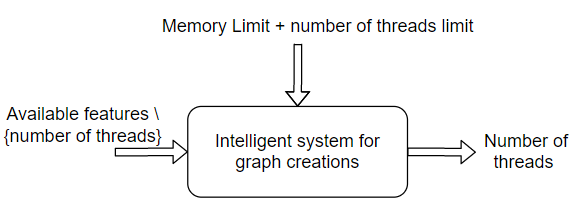
\includegraphics[]{chapters/model.png}
    \caption{Final Model}
    \label{fig:Final Model}
\end{figure}
\FloatBarrier

\section{Conclusion}
In this chapter we presented different stages we went through to create the machine learning models that predict the best strategy to create the graph based on the characteristics of the hardware and details about the graph we want to create. 


